\section{Evaluation}

\subsection{3-Task Theory Evaluation}

For evaluating our three-task theory, we perform four experiments. In the first, we run the tasks on a real-time system and record the miss rate and average freshness of data. Next, we take chains of tasks and a given freshness guarantee, and then check if the produced results are theoretically schedulable. Later, we evaluate how schedulability and utilization may change when altering the desired freshness. Lastly, we examine one task chain and see how the period assignments change when we modify the freshness bound.

For our evaluation we consider uniprocessor systems for simplicity. As described earlier, the evaluation conclusions should largely apply to the multiprocessor systems as well. To test schedulability we use response time analysis for rate monotonic (RM) scheduling and a utilization bound of 1 for earliest deadline first (EDF) scheduling. For our task parameters, we use values from the E3S benchmark\footnote{http://ziyang.eecs.umich.edu/\textasciitilde dickrp/e3s/}. We used all sections of the benchmark, including task sets from the automotive, consumer electronics, networking, office automation, and telecommunications industries.

The task graphs we obtained have between 2 and 10 tasks. To gather as many relevant examples as possible for these special cases, we sometimes combined several serial tasks into one large task, or used several branches of parallel tasks as separate examples for 2-and-3-task evaluations. However, we always included the beginning and ending tasks and some chain from the former to the latter, so that the period values in the benchmark could be used meaningfully. We used WCETs of the first hardware configuration given in the benchmark, and chose BCETs to be half of WCET. We considered communication negligible for evaluation as we global variables between threads of the same process. In total, we collected 26 three-task scenarios and 29 two-task scenarios from the benchmark suite.

For our first experiment, we ran task chains with parameters chosen by our theory on a real system, using a freshness bound of 25\% of the period of the final task so as to have difficult enough chains for meaningful evaluation. We used a Linux testbed\footnote{Ubuntu 14.04, i7-6770HQ CPU, 16GB DDR3 RAM} with either the fixed priority scheduler (SCHED\_FIFO) with priorities set to RM, or the EDF scheduler (SCHED\_DEADLINE). We set up the tasks to run for 99\% of the specified WCET to account for scheduler overhead and context switching. The final task maintains statistics such as average freshness and freshness miss ratio. We ran this for all task sets that passed the respective schedulability test after having parameters selected by our formulation. The average utilization of the task sets was 40.6\% with a low of 1.9\% and a high of 97.4\%. We ran each task set for one minute, which resulted in hundreds to hundreds of thousands of executions of each task. Tasks were all run on the same core with no external loads added.

Under both RM and EDF, all reads by the last task were within the desired freshness bound, i.e. there were no misses, except for far outliers (3-5x the bound) which we discarded as OS, background task, and other outside interferences, as these are far larger than could be reasonably expected. The average percentage of the freshness bound that was consumed before reading a value as well as the average percentage bound consumed for the stalest value were recorded. The top section of Table \ref{table:fresh} summarizes the results. We see that on average the value was well within the maximum bound. Our experiments suggest that RM slightly outperforms EDF when considering average freshness. RM shows the greatest advantages for maximum staleness observed. We believe this is because our 2-and-3-task theory often assigns lower periods, and hence higher priorities, to tasks earlier in the task chain. This may help freshness since producer tasks are executed first which prioritizes pushing newer values though the chain over consuming older values.

\begin{table}[h]
\caption{Comparison of average freshness and miss percentage for task sets under RM and EDF scheduling}
\label{table:fresh}
\begin{center}
	\begin{tabular}{|r|c|c|}
		\hline
		Original Task Set & RM & EDF \\
		\hline
		Freshness Miss Rate (\%) & 0 & 0 \\
		Average Freshness (\% of bound) & 7.8 & 10.3 \\
		Average Max Freshness (\% of bound) & 12.9 & 52.9 \\
		\hline
		Stringent Task Set & RM & EDF \\
		\hline
		Freshness Miss Rate (\%) & 0 & 0 \\
		Average Freshness (\% of bound) & 11.5 & 13.2 \\
		Average Max Freshness (\% of bound) & 26.2 & 81.9 \\
		\hline
	\end{tabular}
\end{center}
\end{table}

The statistics collected in the trial were weighted down by several easily scheduled task sets. To get an idea of how the formulation performed on heavier task sets, we removed task sets where 20\% or less of the bound was consumed on average. In this case the average utilization was 45.2\% with a low of 20.6\% and a high of 83.4\%. We observed the same trend as before where RM outperforms EDF on average, and especially in the maximum staleness metric. The results are shown in the bottom section of Table \ref{table:fresh}.

For our second experiment, we looked at the theoretical schedulability of the task sets. Figure \ref{fig:Schedulability} shows the percentage of task chains which were schedulable using RM or EDF scheduling. The first two sets of bars depict the schedulability percentage when freshness bounds are set equal to the period of the last task in the chain. The second two sets of bars depict the schedulability after we quarter the freshness bound. If the freshness bound is too tight, our formulation will sometimes result in non-positive periods. These cases were included in the evaluation and were considered unschedulable task chains.

\begin{figure}[h]
\centering
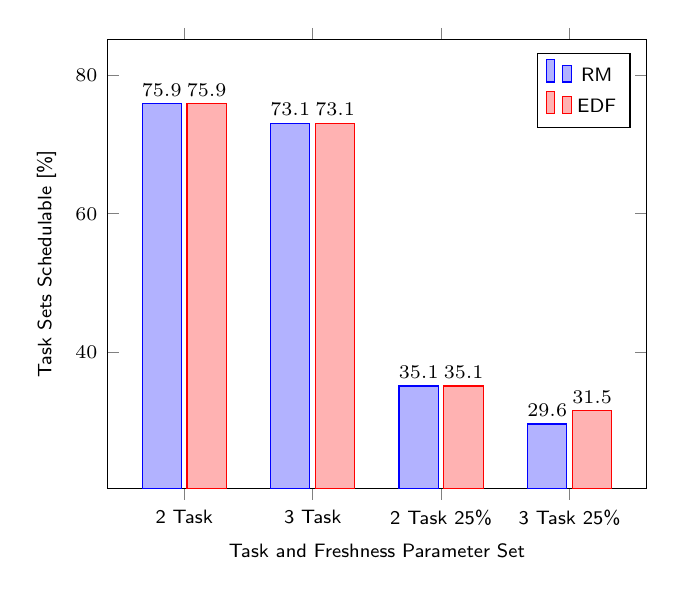
\begin{tikzpicture}[font=\sffamily\scriptsize]
	\begin{axis}[
	ybar,
	enlargelimits=0.2,
	bar width = 0.5cm,
	legend style={legend columns=1},
	legend pos=north east,
	xlabel={Task and Freshness Parameter Set},
	ylabel={Task Sets Schedulable [\%]},
	symbolic x coords={2 Task,3 Task,2 Task 25\%,3 Task 25\%},
	xtick=data,
	nodes near coords,
	nodes near coords align={vertical},
	every node near coord/.append style={color=black, rotate=0, anchor=center,  xshift=0, yshift=5}]
	
	\addplot [forget plot] coordinates {};
	\addplot coordinates {(2 Task,75.9) (3 Task, 73.1) (2 Task 25\%,35.1) (3 Task 25\%,29.6)};
	\addplot coordinates {(2 Task,75.9) (3 Task, 73.1) (2 Task 25\%,35.1) (3 Task 25\%,31.5)};
	
	\legend{RM,EDF}
	\end{axis}
\end{tikzpicture}
\caption{Formulation Schedulability. The first two bar sets show schedulability of task chains with freshness bound equal to period of the last task. The last two bar sets show schedulability when the bound is quartered.}
\label{fig:Schedulability}
\end{figure}

Both schedulers scheduled the same percentage of tasks for the first 3 bar sets and inspection revealed both scheduled the same task chains. The last bar set depicts a task set which showed discrepancy between RM and EDF schedulers, where EDF shows a slight schedulability advantage.

For our third experiment, we choose to repeatedly decrease the freshness bound of each schedulable task set by 10\% from an original freshness bound (equal to the period of the last task in the chain). We then recorded the average utilization and percentage of task chains that are schedulable under EDF. This gives us an idea of the trade-off between freshness and schedulability. The results are charted in the top two lines of Figure \ref{fig:FreshnessChange}. We can see that above about 50\% of the original bound a 10\% decrease in freshness bound results in about 5\% increase in utilization. The areas where utilization decreases (30\% and lower) is due to less task sets being considered, since non-schedulable task chains were omitted from the utilization calculation. We see schedulability is not greatly hindered until we get to around 30\% of the original freshness bound. The primary significance of Figure \ref{fig:FreshnessChange} is that above 30\% of original freshness bound, where the task set stays largely the same, we see only modest increases in utilization when we tighten the freshness bound.

\begin{figure}[h]
\centering
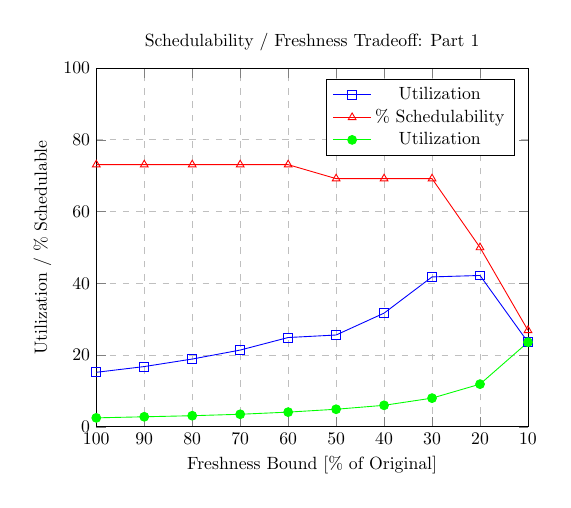
\begin{tikzpicture}[thick,scale=.8, every node/.style={scale=.8}]
\begin{axis}[
title={Schedulability / Freshness Tradeoff: Part 1},
xlabel={Freshness Bound [\% of Original]},
ylabel={Utilization / \% Schedulable},
xmin=10, xmax=100,
ymin=0, ymax=100,
ytick={0,20,40,60,80,100},
xtick={10,20,30,40,50,60,70,80,90,100},
xticklabels={100,90,80,70,60,50,40,30,20,10},
legend pos=north east,
ymajorgrids=true,
xmajorgrids=true,
grid style=dashed,
]

\addplot[
color=blue,
mark=square,
]
coordinates {
	(100,23.6)(90,42.2)(80,41.8)(70,31.7)(60,25.6)(50,24.9)(40,21.4)(30,18.9)(20,16.8)(10,15.2)
};

\addplot[
color=red,
mark=triangle,
]
coordinates {
	(100,26.9)(90,50)(80,69.2)(70,69.2)(60,69.2)(50,73.1)(40,73.1)(30,73.1)(20,73.1)(10,73.1)
};

\addplot[
color=green,
mark=*,
]
coordinates {
	(100,23.6)(90,11.9)(80,8)(70,6)(60,4.9)(50,4.1)(40,3.5)(30,3.1)(20,2.8)(10,2.5)
};

\legend{Utilization,\% Schedulability, Utilization}
\end{axis}
\end{tikzpicture}
\caption{Schedulability, Utilization vs. Freshness.}
\label{fig:FreshnessChange}
\end{figure}

Next we modified the previous experiment by performing the evaluation only on those chains which are schedulable at 10\% of the original freshness bound, to prevent noise due to the differences in the schedulable task chains. In the bottom line of Figure \ref{fig:FreshnessChange} we see a more intuitive curve. It is lower because more difficult chains were not schedulable with very low freshness bounds. Note that a 10\% reduction does not change utilization much if above 50\% of the original freshness bound. We see again that utilization is more greatly affected when below 30\% of the original freshness bound.

\iffalse
\begin{figure}[h]
	\centering
	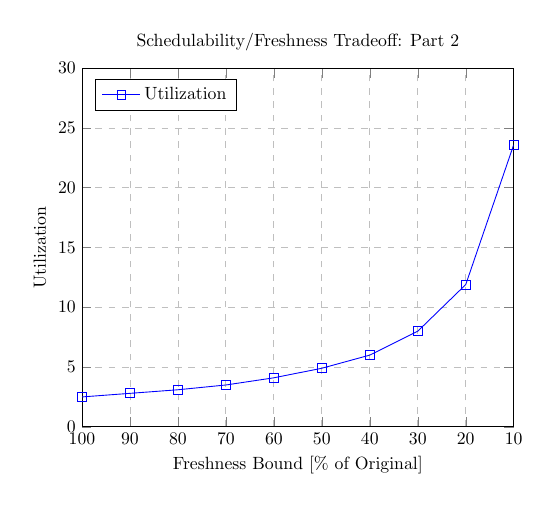
\begin{tikzpicture}[thick,scale=.8, every node/.style={scale=.8}]
	\begin{axis}[
	title={Schedulability/Freshness Tradeoff: Part 2},
	xlabel={Freshness Bound [\% of Original]},
	ylabel={Utilization},
	xmin=10, xmax=100,
	ymin=0, ymax=30,
	ytick={0,5,10,15,20,25,30},
	xtick={10,20,30,40,50,60,70,80,90,100},
	xticklabels={100,90,80,70,60,50,40,30,20,10},
	legend pos=north west,
	ymajorgrids=true,
	xmajorgrids=true,
	grid style=dashed,
	]
	
	\addplot[
	color=blue,
	mark=square,
	]
	coordinates {
		(100,23.6)(90,11.9)(80,8)(70,6)(60,4.9)(50,4.1)(40,3.5)(30,3.1)(20,2.8)(10,2.5)
	};
	
	\legend{Utilization}
	\end{axis}
	\end{tikzpicture}
	\caption{Freshness vs. Utilization. Result for task chains that remain schedulable even with a freshness bound 10\% of the consuming task's period.}
	\label{fig:FreshnessChangeControlled}
\end{figure}
\fi

For our fourth experiment, we chose a three task chain which was schedulable with freshness bound of 10\% of the period of the last task. This chain was from the automotive industry. We then calculated the periods of the input tasks according to our theory in increments of 10\% of the original freshness bound. We'll name our tasks in the chain as $A \to B \to C$. In this case, task $A$ has a WCET of $50$, task $B$ a WCET of $155$, and task $C$ a period and WCET of $15000$ and $50$ milliseconds respectively. BCETs were set to half of WCET. How the assigned periods of tasks $A$ and $B$ change to reflect the change in freshness bound is displayed in Figure \ref{fig:TaskSet4}. We see that changes in freshness causes linear changes in the periods of both tasks to account for the new bound.

\begin{figure}[h]
	\centering
	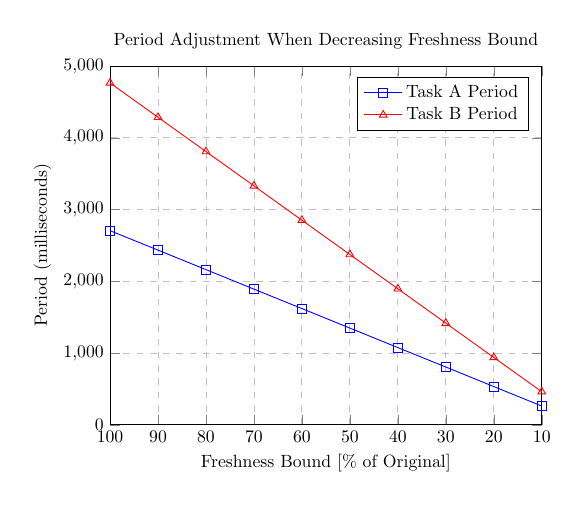
\begin{tikzpicture}[thick,scale=.8, every node/.style={scale=.8}]
	\begin{axis}[
	title={Period Adjustment When Decreasing Freshness Bound},
	xlabel={Freshness Bound [\% of Original]},
	ylabel={Period (milliseconds)},
	xmin=10, xmax=100,
	ymin=0, ymax=5000,
	ytick={0,1000,2000,3000,4000,5000},
	xtick={10,20,30,40,50,60,70,80,90,100},
	xticklabels={100,90,80,70,60,50,40,30,20,10},
	legend pos=north east,
	ymajorgrids=true,
	xmajorgrids=true,
	grid style=dashed,
	]
	
	\addplot[
	color=blue,
	mark=square,
	]
	coordinates {
		%(10,0.34)(20,0.66)(30,0.99)(40,1.30)(50,1.62)(60,1.94)(70,2.26)(80,2.58)(90,2.89)(100,3.21)
		(100,262)(90,534)(80,806)(70,1077)(60,1349)(50,1621)(40,1892)(30,2164)(20,2436)(10,2707)
	};
	
	\addplot[
	color=red,
	mark=triangle,
	]
	coordinates {
		%(10,0.23)(20,0.41)(30,0.59)(40,0.77)(50,0.95)(60,1.13)(70,1.31)(80,1.49)(90,1.67)(100,1.85)
		(100,462)(90,940)(80,1418)(70,1897)(60,2375)(50,2853)(40,3332)(30,3810)(20,4288)(10,4767)
	};
	
	\legend{Task A Period, Task B Period}
	\end{axis}
	\end{tikzpicture}
	\caption{Freshness vs. Periods. Using one task chain that is schedulable with a freshness bound at 10\% of task $C$'s period, we plot how our formulation assigns periods tasks $A$ and $B$ to maintain freshness.}
	\label{fig:TaskSet4}
\end{figure}

\subsection{Optimization Formulation Evaluation}

To evaluate the optimization formulation we implemented the described optimization problems in MATLAB. In our figures we will denote the general formulation as ``G-'' and the RM-targeting formulation as ``R-'' followed by the scheduler used. For example, G-RM denotes data using solutions from the general formulation ran under a RM scheduler.

For each chain length, we randomly generated tasks with between 1 and 5 units of work for their BCET, and added another 1 to 5 to the BCET to determine the WCET. We then generated an end-to-end deadline equal to the sum of the task WCETs multiplied by a random integer between 3 and 10, in order to add slack to the system that depends on the number of tasks and their execution lengths so that chain lengths and WCETs do not adversely affect the results. All random variables were drawn from a uniform distribution. We used the same necessary and sufficient schedulability uniprocessor tests for RM and EDF as before. Figure \ref{fig:OptimizationOptimizationByChainLength} depicts the schedulability of the generated task sets. Each bar represents the percentage of 1000 generated task sets that were schedulable. Note the same 1000 task sets were used for each formulation-scheduler combination.

\begin{figure}[h]
	\centering
	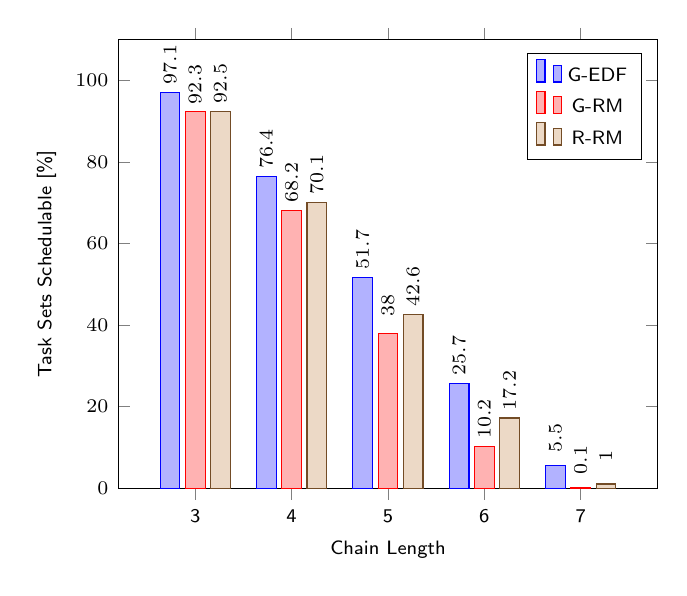
\begin{tikzpicture}[font=\sffamily\scriptsize]
	\begin{axis}[
	ybar,
	enlargelimits=0.2,
	enlarge y limits={upper=0},
	bar width = 0.25cm,
	legend style={legend columns=1},
	legend pos=north east,
	xlabel={Chain Length},
	ylabel={Task Sets Schedulable [\%]},
	symbolic x coords={3,4,5,6,7},
	ymin=0, ymax=100,
	xmin=3, xmax=7,
	xtick=data,
	nodes near coords,
	nodes near coords align={vertical},
	every node near coord/.append style={color=black, rotate=90, anchor=center, xshift=10, yshift=0}]
	
	\addplot [forget plot] coordinates {};
	\addplot coordinates {(3,97.1) (4, 76.4) (5,51.7) (6,25.7) (7,5.5)};
	\addplot coordinates {(3,92.3) (4, 68.2) (5,38.0) (6,10.2) (7,0.1)};
	\addplot coordinates {(3,92.5) (4, 70.1) (5,42.6) (6,17.2) (7,1.0)};
	
	\legend{G-EDF,G-RM,R-RM}
	\end{axis}
	\end{tikzpicture}
	\caption{Schedulability of Optimization Results with Differing Chain Lengths.}
	\label{fig:OptimizationOptimizationByChainLength}
\end{figure}

We see that EDF performs more favorably in terms of schedulability. However, we do see a small improvement in RM schedulability when we use our RM-targeted formulation. This improvement seems to increase with chain length.

\iffalse
\begin{figure}[h]
	\centering
	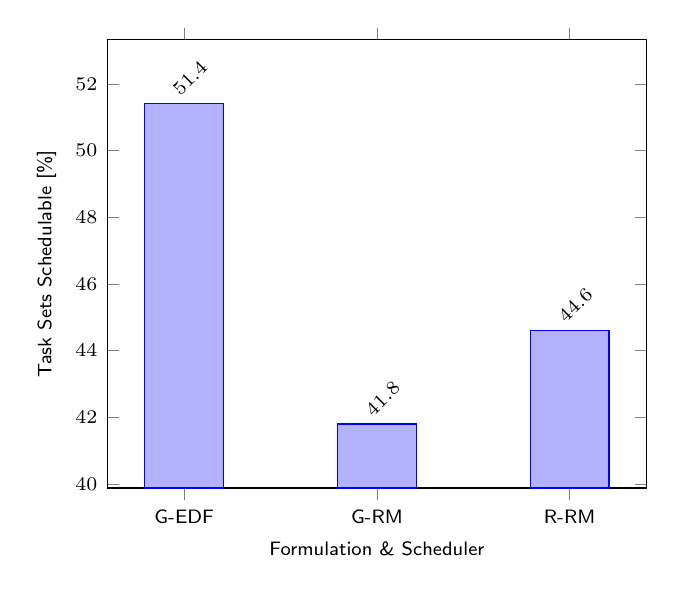
\begin{tikzpicture}[font=\sffamily\scriptsize]
	\begin{axis}[
	ybar,
	enlargelimits=0.2,
	bar width = 1cm,
	legend style={at={(0.5,1.15)},
		anchor=north,legend columns=-1},
	xlabel={Formulation \& Scheduler},
	ylabel={Task Sets Schedulable [\%]},
	symbolic x coords={G-EDF,G-RM,R-RM},
	xtick=data,
	nodes near coords,
	nodes near coords align={vertical},
	every node near coord/.append style={color=black, rotate=45, anchor=center, xshift=8, yshift=5}]
	
	\addplot [forget plot] coordinates {};
	\addplot coordinates {(G-EDF, 51.4) (G-RM,41.8) (R-RM,44.6)};
	
	\end{axis}
	\end{tikzpicture}
	\caption{Schedulability of Optimization Results with Mixed Chain Lengths Between 3 and 7 Inclusive.}
	\label{fig:OptimizationOptimizationRandomChains}
\end{figure}
\fi

%Using the same generation methods as above but instead randomly generating chain lengths between 3 and 7, we saw the schedulability depicted in Figure \ref{fig:OptimizationOptimizationRandomChains}.

To show that our method is applicable to longer chain lengths and to analyze the scaling ability of the method according to the task set, we ran the above optimization and analysis but with a harder and easier task sets. More precisely, we kept the same task set as depicted in Figure \ref{fig:OptimizationOptimizationByChainLength} but with the end-to-end freshness deadline either halved (twice as hard) or doubled (half as hard). The results of the latter are shown in Figure~\ref{fig:OptimizationOptimizationByChainLengthEasy}.

\iffalse
\begin{figure}[h]
	\centering
	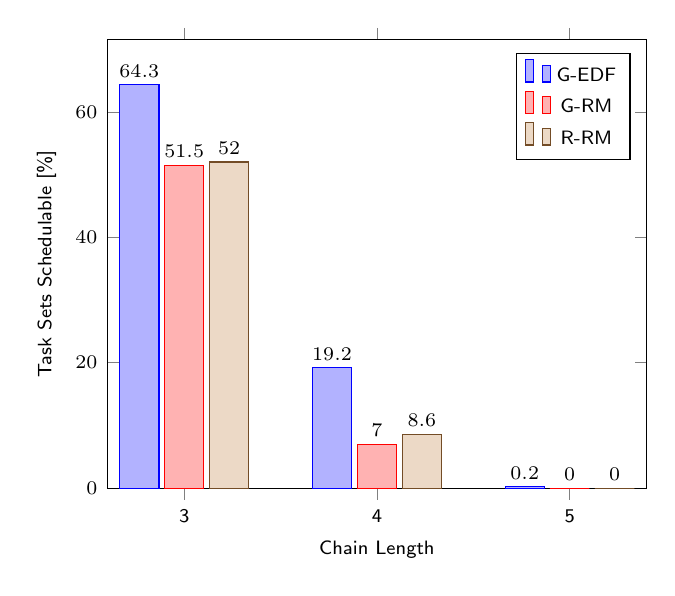
\begin{tikzpicture}[font=\sffamily\scriptsize]
	\begin{axis}[
	ybar,
	enlargelimits=0.2,
	enlarge y limits={upper=0},
	bar width = 0.5cm,
	legend style={legend columns=1},
	legend pos=north east,
	xlabel={Chain Length},
	ylabel={Task Sets Schedulable [\%]},
	symbolic x coords={3,4,5},
	ymin=0, ymax=65,
	xmin=3, xmax=5,
	xtick=data,
	nodes near coords,
	nodes near coords align={vertical},
	every node near coord/.append style={color=black, rotate=0, anchor=center, xshift=0, yshift=5}]
	
	\addplot [forget plot] coordinates {};
	\addplot coordinates {(3,64.3) (4, 19.2) (5,0.2)};
	\addplot coordinates {(3,51.5) (4, 7.0) (5,0.0)};
	\addplot coordinates {(3,52.0) (4, 8.6) (5,0.0)};
	
	\legend{G-EDF,G-RM,R-RM}
	\end{axis}
	\end{tikzpicture}
	\caption{Schedulability of Optimization Results with Differing Chain Lengths, with deadlines halved. This approximates a twice as difficult task set.}
	\label{fig:OptimizationOptimizationByChainLengthHard}
\end{figure}
\fi

\begin{figure}[h]
	\centering
    %\begin{adjustbox}{width=0.85\textwidth}
	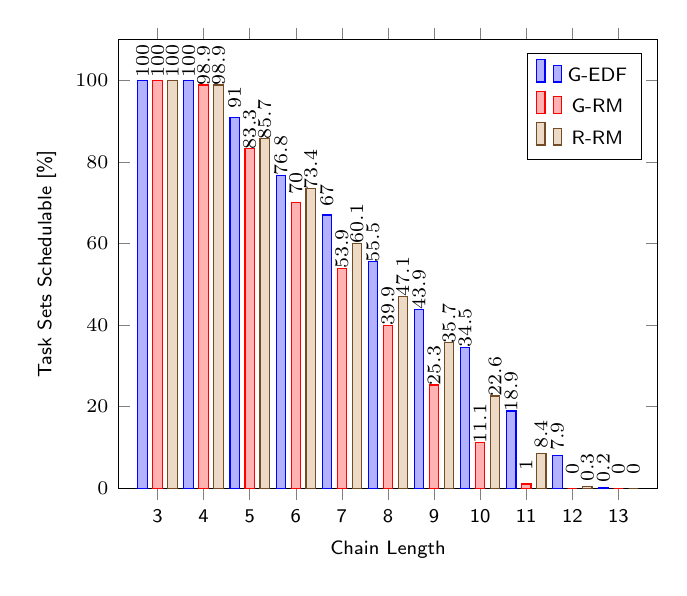
\begin{tikzpicture}[font=\sffamily\scriptsize]
	\begin{axis}[
	ybar,
	enlargelimits=0.2,
    enlarge x limits={abs=0.5cm},
    enlarge y limits={upper=0},
	bar width = 0.12cm,
	legend style={legend columns=1},
	legend pos=north east,
	xlabel={Chain Length},
	ylabel={Task Sets Schedulable [\%]},
	symbolic x coords={3,4,5,6,7,8,9,10,11,12,13},
	ymin=0, ymax=100,
	xmin=3, xmax=13,
	xtick=data,
	nodes near coords,
	nodes near coords align={vertical},
	every node near coord/.append style={color=black, rotate=90, anchor=center, xshift=7, yshift=0}]
	
	\addplot [forget plot] coordinates {};
	\addplot coordinates {(3,100.0) (4, 100.0) (5,91.0) (6,76.8) (7,67.0) (8,55.5) (9,43.9) (10,34.5) (11,18.9) (12,7.9) (13,0.2)};
	\addplot coordinates {(3,100.0) (4, 98.9) (5,83.3) (6,70.0) (7,53.9) (8,39.9) (9,25.3) (10,11.1) (11,1.0) (12,0.0) (13,0.0)};
	\addplot coordinates {(3,100.0) (4, 98.9) (5,85.7) (6,73.4) (7,60.1) (8,47.1) (9,35.7) (10,22.6) (11,8.4) (12,0.3) (13,0.0)};
	
	\legend{G-EDF,G-RM,R-RM}
	\end{axis}
	\end{tikzpicture}
        %\end{adjustbox}
	\caption{Schedulability of Optimization Results with Differing Chain Lengths: Deadlines Doubled.}
	\label{fig:OptimizationOptimizationByChainLengthEasy}
\end{figure}

We can see that the trend remains about linear in schedulability after the modification. Similar scaling was seen in the more difficult task set but the figure is omitted due to space considerations. These experiments suggest that the formulation's schedulability generally scales inversely with chain length. There is no chain length from our trials that causes the schedulability to unexpectedly drop. It appears that our formulation can handle approximately twice the chain length for each halving in difficulty and vice versa, with some small losses due to pessimism.

In our final evaluation we again referenced the E3S benchmark to evaluate real-world performance with multiple chain lengths. We chose chains that all three formulations could schedule. We ran the chains and collected freshness data as we did in the three-task theory evaluation. The results are summarized in the Table \ref{table:freshess_e3s}.

\begin{table}[h]
	\caption{Comparison of freshness for task chains under RM or EDF scheduling using results from the general or RM-specific formulation.}
	\label{table:freshess_e3s}
	\begin{center}
		\begin{tabular}{|r|c|c|c|}
			\hline
			& G-EDF & G-RM & RM-RM \\
			\hline
			Average Freshness (\% of bound) & 13.73 & 4.77 & 4.77 \\
			Average Max Freshness (\% of bound) & 56.20 & 33.75 & 31.89 \\
			\hline
		\end{tabular}
	\end{center}
\end{table}

RM scheduling provided better average and maximum staleness when executing the results from either optimization, further supporting that for real-world task sets similar to the E3S benchmark, RM provides greater freshness than EDF.

Overall, our optimization formulation seems adequate for short to moderate chain lengths. We suspect that many real-life systems use chain lengths within the evaluated ranges, including all of the E3S benchmark chains. As far as optimization efficiency, the optimization problem finished on average in less than a second. This suggests that the scaling of the optimization problem would not be a limiting factor in the use of our system.
